\documentclass[10pt,a4paper]{article}
\usepackage[utf8]{inputenc}
\usepackage[portuguese]{babel}
\usepackage[T1]{fontenc}
\usepackage{amsmath}
\usepackage{amsfonts}
\usepackage{amssymb}
\usepackage[a4paper, total={6in, 8in}]{geometry}
\usepackage{graphicx}
\usepackage{float}
\usepackage{caption}
\usepackage{pdfpages}
\usepackage{multirow} 
\usepackage{indentfirst}
\setcounter{tocdepth}{4}
\setcounter{secnumdepth}{4}


\numberwithin{equation}{section}
\addto\captionsenglish{
\renewcommand{\figurename}{Figura}
\renewcommand{\tablename}{Tabela}
}

\newcount\colveccount
\newcommand*\colvec[1]{
        \global\colveccount#1
        \begin{pmatrix}
        \colvecnext
}
\def\colvecnext#1{
        #1
        \global\advance\colveccount-1
        \ifnum\colveccount>0
                \\
                \expandafter\colvecnext
        \else
                \end{pmatrix}
        \fi
}


\usepackage{fancyhdr}
\pagestyle{fancy}
%\fancyhead[LE,RO]{\textsl{\rightmark}}
\fancyhead[LE,RO]{\thepage}
\fancyhead[LO,RE]{\textsl{\leftmark}}
\fancyfoot[C]{}


\begin{document}
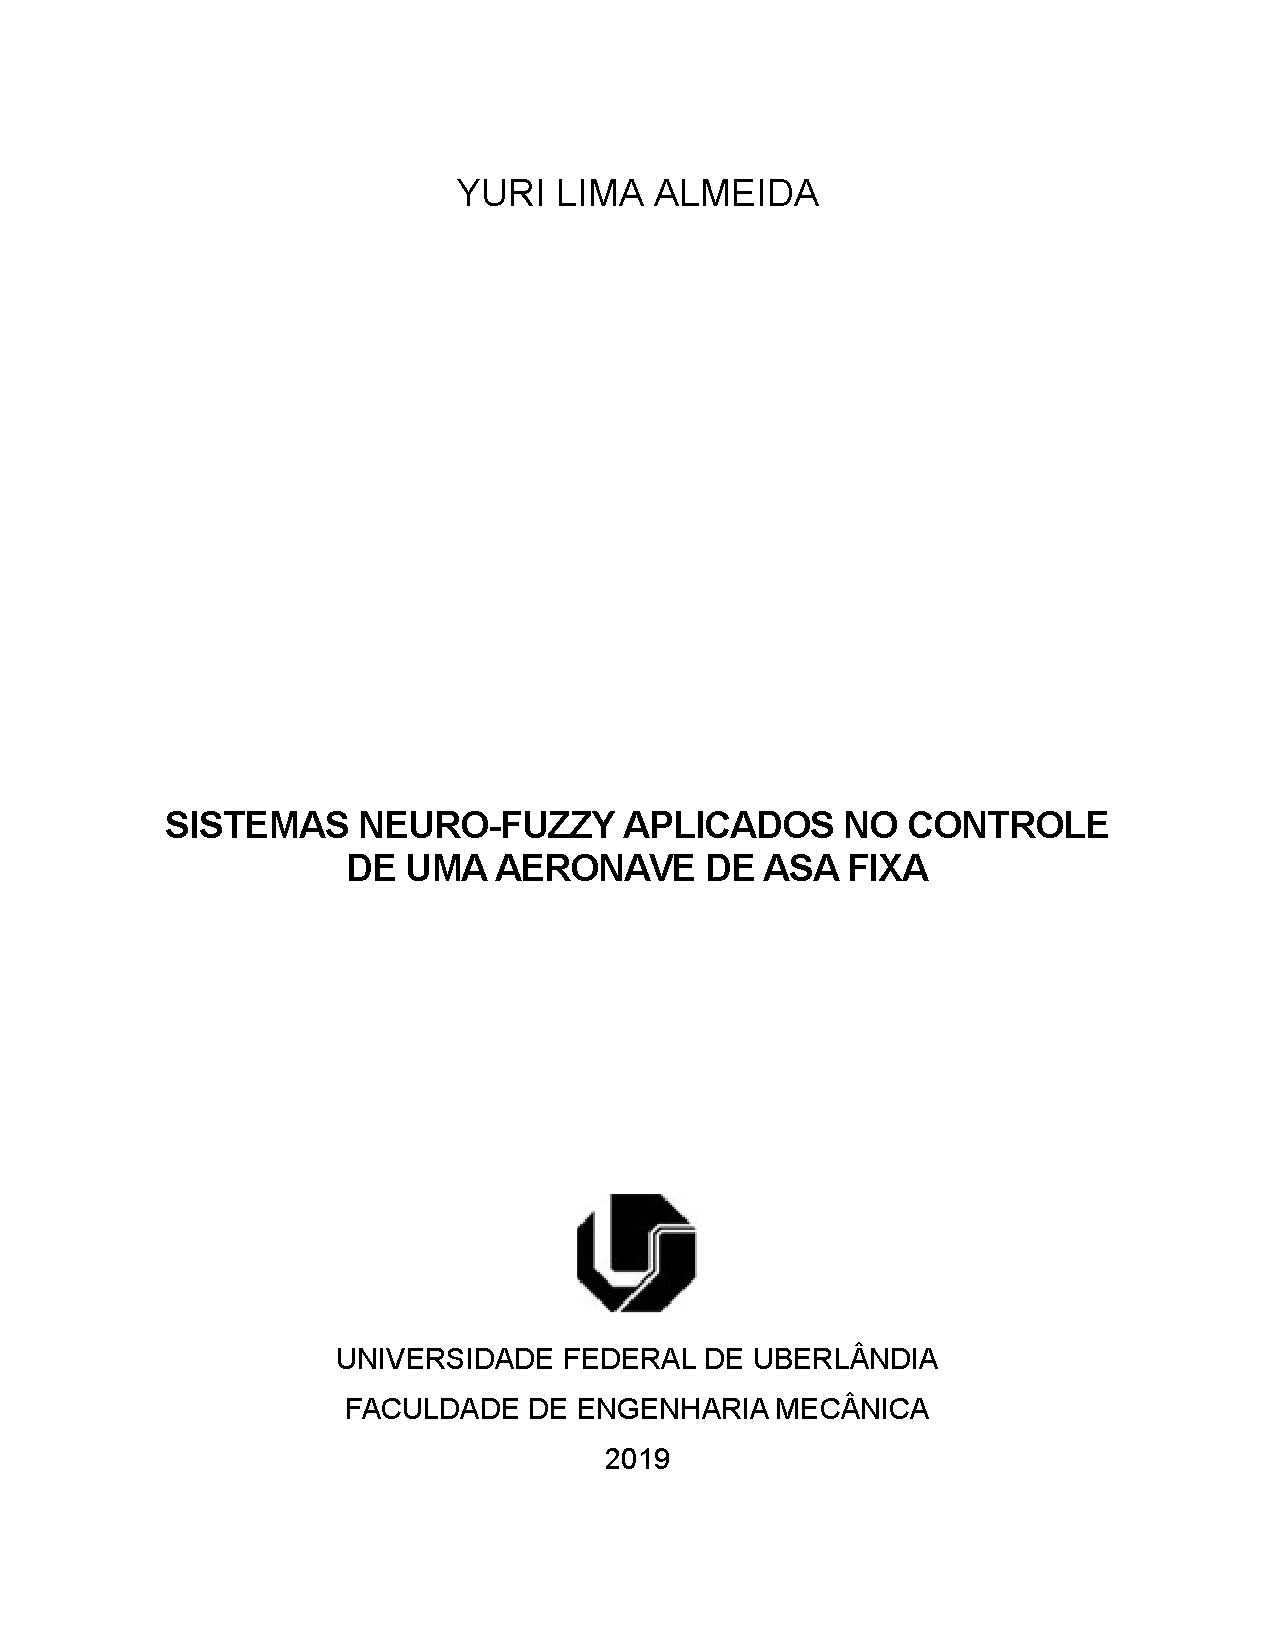
\includepdf[page=-]{2pag.pdf} 
\pagenumbering{roman}
\section*{Agradecimentos}

\par 

\newpage

\section*{Resumo}
\par  de controle da aeronave duran


\newline
\newline
\newline
\textbf{Palavras-chave:} controle inteligente, Sistemas Neuro-fuzzy, Evolução Diferencial, Recozimento Simulado, desempenho, estabilidade.

\newpage
\section*{Abstract}
\par The loss of the aircraft’s control during the flight is the main cause of deaths in plane crashes. For this reason, it is of great importance to develop an efficient controller, that many times cannot be obtained through the basic techniques. In this project it is performed the control of a fixed-wing airplane using neuro-fuzzy systems, with parameters obtained through Differential Evolution and from Simulated Annealing.It is used MatLab® \textit{software} to obtain the controller and to evaluate the system’s performance and stability.The obtained results indicate that the controller is capable of compensating eventual system disturbances. Furthermore, the Simulated Annealing shows a shorter time of execution to find the optimum controller, by contrast, this method shows a higher standard deviation of the results, which suggests a higher randomness and imprecision than the Differential Evolution method.
\newline
\newline
\newline
\textbf{Keywords}: intelligent control, Neuro-fuzzy systems, Differential Evolution, simulated annealing, performance, stability.
\newpage
\listoffigures
\newpage
\listoftables
\newpage
\section*{Lista de Símbolos}

\noindent $a_i^l$  - variável de saída do neurônio i da RNA\\
$b_i^l$ - bias associado ao neurônio i\\
$Cf$ - função custo\\
$C_{i,k}$ - vetor de cruzamento da Evolução Diferencial \\
CR – taxa de cruzamento\\
dt – tempo de amostragem \\
$E^k$  - energia interna da solução k\\
F – fator de perturbação\\
$f_{obj}$ - função objetivo\\
h  - altitude\\
$I_{CG}$ - momento de inércia do centro de gravidade da aeronave\\
$I_x$  - momento de inércia em relação ao eixo x\\
$I_y$ - momento de inércia em relação ao eixo y\\
$I_z$ - momento de inércia em relação ao eixo z\\
$I_{xz}$ – produto de inércia relativamente a x e z\\
L – momento de rolagem da aeronave\\
$L_0$ - valor nominal de momento de rolagem\\
M – momento de arfagem da aeronave\\
$M_0$ - valor nominal de momento de arfagem\\
m - massa do sistema\\
N – momento de guinada da aeronave\\
$N_0$ - valor nominal de momento de guinada\\
$n_e$ - número de elementos dos vetores\\
P – velocidade angular de rolagem da aeronave\\
$P_0$ – valor nominal da velocidade angular de rolagem\\
p - perturbação da velocidade angular de rolagem\\
$p_{RM}$ – probabilidade em se aceitar um ponto com maior energia interna\\
Q – velocidade angular de arfagem da aeronave\\
$Q_0$ - valor nominal da velocidade angular de arfagem\\
q - perturbação da velocidade angular de arfagem\\
R – velocidade angular de guinada da aeronave\\
$R_0$ - valor nominal da velocidade angular de guinada\\
r – perturbação da velocidade angular de guinada\\
$R_{x,\Phi}$  - matriz de transformação do sistema do corpo para o sistema inercial na direção x\\
$R_{x,\Phi}^\top$  - matriz de transformação do sistema inercial para o sistema do corpo na direção x \\
$R_{y,\Theta}$  - matriz de transformação do sistema do corpo para o sistema inercial na direção y\\
$R_{y,\Theta}^\top$  - matriz de transformação do sistema inercial para o sistema do corpo na direção y\\
$R_{z,\Psi}$  - matriz de transformação do sistema do corpo para o sistema inercial na direção z\\
T – constante de tempo\
$T_a$ - tempo de acomodação do sistema\\
$T^k$ – temperatura no instante k\\
U – velocidade longitudinal da aeronave\\
$U_0$ - valor nominal de velocidade longitudinal\\
u - perturbação da velocidade longitudinal \\
V – Velocidade lateral da aeronave\\
$V_0$ - valor nominal de velocidade lateral\\
$V_{i,k}$ - vetor de mutação da Evolução Diferencial\\
v - perturbação da velocidade lateral\\
W – velocidade vertical  da aeronave\\
$W_0$ - valor nominal de velocidade vertical \\
w – perturbação da velocidade vertical\\
$w_{ij}^l$ – peso sináptico associado ao neurônio i\\
X – força longitudinal \\
$X_0$ - valor nominal de força longitudinal\\
$X_E$ – posição x do eixo inercial da terra\\
$X_{i,k}$ - vetor de inicialização da Evolução Diferencial\\
$x_k$ - valor de x (variável qualquer) no instante k\\
$x_{ref}$ – valor de x (variável qualquer) de referência\\
Y – força transversal \\
$Y_0$ - valor nominal de força transversal\\
$Y_E$ - posição y do eixo inercial da terra\\
$y_r$ – parâmetro de controle\\
$y_s$ - saída do controlador\\
Z – força vertical \\
$Z_0$ - valor nominal de força vertical \\
$Z_E$  - posição z do eixo inercial da terra\\
$\alpha$ – fator utilizado no decaimento da temperatura no Recozimento Simulado\\
$\delta ail$ - deflexão do aileron da aeronave\\
$\delta L$ - perturbação do momento de rolagem\\
$\delta lem$ - deflexão do leme da aeronave \\
$\delta M$ – perturbação do momento de arfagem\\
$\delta N$ - perturbação do momento de guinada\\
$\delta pr$ - deflexão do profundor da aeronave \\ 
$\delta X$ - perturbação da força longitudinal\\
$\delta Y$ - perturbação da força transversal\\
$\delta Z$ - perturbação da força vertical\\
$\Theta$ – ângulo de arfagem da aeronave\\
$\Theta_0$ - valor nominal do ângulo de arfagem\\
$\theta$ - perturbação do ângulo de arfagem\\
$\sigma$ – função de ativação da rede neural\\
$\overrightarrow{\tau}_1$ – forças do sistema\\
$\overrightarrow{\tau}_2$ - momentos do sistema\\
$\Phi$ - ângulo de rolagem da aeronave\\
$\Phi_0$ - valor nominal do ângulo de rolagem\\
$\phi$ – perturbação do ângulo de rolagem\\
$\Psi$ – ângulo de guinada da aeronave\\
$\Psi_0$ - valor nominal do ângulo de guinada\\
$\psi$ - perturbação do ângulo de guinada\\

\newpage

\section*{Glossário}

\noindent ANFIS – Sistema de Inferência Neuro-\textit{Fuzzy} Adaptativo (\textit{Adaptative neuro-fuzzy inference system})\\
ANN – Redes Neurais Artificiais (\textit{Artificial Neural Network})\\
CENIPA - Centro de Investigação e Prevenção de Acidentes Aeronáuticos\\
FIS – Sistema de Inferência \textit{Fuzzy} (\textit{Fuzzy Inference System})\\
IA – Inteligência Artificial\\
PID - Proporcional-Integral-Derivativo\\
RNA – Rede Neural Artificial\\
SBRF – Sistema Baseado em Regras \textit{Fuzzy}\\
VANTS – Veículos aéreos não tripulados\\







\newpage
\tableofcontents
\newpage
\pagenumbering{arabic}
\setcounter{page}{12}
\section{Introdução}
%Nos países que possuem grande extensão territorial, como é o caso do Brasil, se faz necessário uma estrutura de transporte que permite a alta mobilidade geográfica da população e uma facilidade na distribuição de mercadorias, de forma a se vencer o relevo sem muita dificuldade. Observa-se que o desenvolvimento econômico do país nas últimas décadas tem como conseqüência um crescimento considerável da aviação brasileira. De acordo com estudos realizados pelo CENIPA (Cenipa, 2017) (Centro de Investigação e Prevenção de Acidentes Aeronáuticos), nos últimos 10 anos (2008-2017) houve 1187 acidentes aéreos registrados, com média de 119 acidentes por ano. O maior percentual de acidentes, representando $53\%$ conforme Fig., tem como principais causas:

\begin{itemize}
\item Falha do motor em vôo;
\item Perda de controle no solo;
\item Perda de controle em vôo;
\end{itemize}


\par Além disso, registros mostram que o número de vítimas fatais é considerável. Dessa forma, é interessante que se desenvolva um controle de aeronaves que tenha como objetivo diminuir a ocorrência dos acidentes, garantindo assim, uma maior segurança para quem utiliza esse meio de transporte.
\par Devido a sua simplicidade e robustez, o controlador PID (Proporcional Integral Derivativo) é o principal método de controle utilizado hoje no mundo. Porém, quando dispomos de processos não lineares, que possuem variantes no tempo, estes controladores podem não responder de uma forma satisfatória (Gianelli,2013). Exitem então outras técnicas de controle capazes de se adaptar ao sistema complexo e fornecer uma resposta otimizada, uma delas é utilizando a Inteligência Artificial (IA) para a obtenção do controlador e sua estrutura matemática.
\par A Inteligência artificial, sendo um ramo de pesquisa da ciência da computação, tem como objetivo construir algoritmos capazes de simular a inteligência dos seres vivos e aplicá-la no processamento de informações. Estes algoritmos devem, a partir da combinação de grandes quantidades de dados, de forma rápida e interativa, aprender com informações ou padrões apresentados nos dados e tomar decisões. Algumas tecnologias englobadas dentro do ramo da IA são:


\begin{itemize}
\item \textbf{Rede neural}: estrutura composta de unidades interconectadas, denominadas neurônios. Estas unidades processam os dados de entrada e retransmitem às unidades seguintes, até se obter a resposta desejada.
\item \textbf{Machine learning}: processo de automatização da construção de modelos analíticos que utiliza da técnica de redes neurais aliada à estatística, pesquisa de operações e física para que sejam encontrados pontos de interesse nos dados.
\item \textbf{Visão computacional}: utiliza do reconhecimento de padrões em imagens para identificar e interpretar o que existe ao redor.
\end{itemize}

\par Hoje existem alguns avanços na área, como a criação de uma tecnologia de aprendizagem desenvolvida por cientistas na Universidade de Berkley, Califórnia, que permite aos robôs que os mesmos imaginem o futuro de suas ações, possibilitando a  tomada de decisões a partir do futuro previsto (O FUTURO DAS COISAS, 2017).
\par Neste projeto, a IA é de grande importância para criar um controlador que tem como principal característica a adaptabilidade, obtendo os parâmetros de forma eficaz e rápida. As técnicas utilizadas para a criação do controlador são apresentadas abaixo:

\begin{itemize}
\item \textbf{Sistema Neuro-\textit{fuzzy}}: sistema de hibridização das técnicas de modelagem de Redes Neurais e Sistemas de Inferência \textit{Fuzzy}.
\item \textbf{Evolução Diferencial}: método robusto de minimização de funções, utilizado para obtenção dos parâmetros do Sistema Neuro-\textit{fuzzy}. 
\item \textbf{Recozimento Simulado}: método de minimização de funções originado da analogia do recozimento de metais, também utilizado para obtenção dos parâmetros do Sistema \textit{Neuro-\textit{fuzzy}}.
\end{itemize}

\par O projeto a seguir contará com: objetivos, justificativa, fundamentação teórica, onde será realizada uma breve revisão bibliográfica acerca do tema, metodologia, desenvolvimento, resultados e discussões, conclusão e trabalhos futuros e referências bibliográficas.

\newpage

\section{Objetivos}

\par Esta monografia está inserida em um projeto desenvolvido por alunos, professores, mestrandos e doutorandos da Universidade Federal de Uberlândia que tem como objetivo principal o desenvolvimento de um controlador adaptativo inteligente aplicado a uma aeronave Cessna 172 em escala reduzida, possibilitando sua total autonomia durante os vôos, que é garantida pela estabilidade e pelo desempenho do controlador.
\par Como objetivos específicos, tem-se a utilização de técnicas neuro-\textit{fuzzy} frequentemente utilizada na inteligência artificial e, a obtenção dos parâmetros deverá ser feita utilizando dois métodos diferentes (Evolução Diferencial e Recozimento Simulado), os quais serão comparados ao fim deste trabalho. Também será realizada a avaliação do sistema quando submetido à perturbações em suas variáveis de estado.


\newpage

\section{Justificativa}

% \par De acordo com dados apresentados pelo CENIPA (Centro de Investigação e Prevenção de Acidentes Aeronáuticos, observados na Fig.\ref{acidente}), uma das principais causas para os acidentes aéreos é a perda de controle da aeronave durante o vôo. A aplicação de algoritmos de controle mais eficientes, visando melhorias em quesitos como performance e estabilidade, ajudaria a diminuir tais estatísticas, tornando aviões comerciais e VANTS mais seguros. Além disso, as vantagens do uso de controle inteligente se dão pela capacidade de adaptação do mesmo, oferecendo robustez às mudanças de cenários, como por exemplo, instabilidades climáticas, chuvas e vento forte.
\par É importante que, na graduação, tenha-se a aplicação na prática das disciplinas apresentadas de forma teórica e didática durante o curso. O projeto em questão engloba desde disciplinas mais básicas até as mais complexas, como Programação Aplicada à Engenharia, Controle de Sistemas Lineares, Controle Digital de Sistemas e Inteligência Computacional (oferecida como optativa), cumprindo a proposta de um Projeto de Fim de Curso.
\par Finalmente, vislumbrando o desenvolvimento da pesquisa nessa área, esse projeto está inserido na tese de doutorado do aluno Bruno Luiz Pereira, que vem com uma proposta inovadora e gerando uma grande e importante contribuição para o meio científico.


\newpage

\section{Fundamentação Teórica}

\subsection{Mecânica do Vôo}

\par Esse item tem como objetivo fornecer uma breve introdução à modelagem dinâmica de uma aeronave. Para um estudo mais aprofundado pode-se utilizar como referência (Fossen, 2011) e (Roskam, 1997).
\par De acordo com Machini (2016) as equações do movimento para qualquer configuração tradicional de aeronave como helicópteros e aviões, podem ser derivadas a partir da segunda lei de Newton aplicada a corpos rígidos com 6 graus de liberdade, possuindo assim 3 graus de translação e 3 graus de rotação. Sendo assim, utiliza-se para a modelagem dois referenciais, sendo eles: um referencial inercial fixo à terra denotado por $I_{cs}$ e outro baricêntrico fixo à aeronave capaz de transladar e rotacionar junto com a mesma $B_{cs}$.  Uma vez que as forças e momentos, sejam elas aerodinâmicas ou inerciais, atuam no corpo, as equações do movimento são derivadas em relação ao referencial $B_{cs}$. Por conseqüência pode-se definir qualquer vetor escrito no referencial $B_{cs}$ no referencial $I_{cs}$ utilizando os ângulos de Euler. Estes representam a atitude da aeronave, que é definida por: arfagem ($\Theta$), rolagem ($\Phi$) e guinada ($\Psi$).
\par A definição das velocidades, posição ou ângulos e forças ou momentos podem ser visualizados a partir das Eq. (4.1), (4.2) e (4.3).


\newpage
\section{Conclusão e trabalhos futuros}

\par O trabalho apresenta a aplicação de técnicas de controle inteligente na análise e controle do avião Cessna 172 em escala real, para isso faz-se necessária a realização da modelagem dinâmica da aeronave e do sistema de controle utilizado. São realizadas simulações envolvendo dois métodos diferentes de otimização, utilizados na obtenção dos parâmetros do controlador.
\par Observa-se que, para todas as análises de sistemas realizadas, o controlador agiu de forma efetiva, produzindo na entrada uma resposta evoluindo ao encontro do ponto de referencia definido. 
\par Ambos os métodos de otimização utilizados se mostraram capazes de encontrar os parâmetros para se obter um controlador otimizado, porém, demonstraram características que diferem entre si e devem ser analisadas conforme comportamento e necessidades do problema a ser estudado. A Evolução Diferencial é um método que se mostra assertivo no cálculo do controlador, produzindo menores erros e uma constância na apresentação dos resultados, com desvio padrão relacionado ao erro RMS igual a zero para diferentes simulações. Apesar disso, possui um tempo de execução maior, comprometendo a eficiência do controlador na hipótese de ser utilizado em aplicação \textit{online}.  O Recozimento Simulado apresenta maior dispersão no erro RMS, podendo influenciar na resposta do controlador a cada simulação realizada. Em contrapartida, a média e o desvio padrão do tempo de execução do método é inferior, viabilizando sua utilização em aplicação \textit{online}.
\par Vislumbrando trabalhos futuros, pretende-se observar o comportamento dos dois métodos apresentados quando utilizadas outras funções objetivo, a fim de melhorar a resposta do sistema controlado. Ainda, o desenvolvimento do controle de forma \textit{online} se faz pertinente, uma vez que confere a adaptabilidade do controlador a condições extremas que modificam o comportamento do sistema.  

\newpage

\section{Referências Bibliográficas}

\par BATISTA, Rafael Gomes; MENEGHETTI, Carlos Renato. Sistema comparativo de controle inteligente de nível aplicado às lógicas \textit{fuzzy} e pid. Unisal,  jun. 2018.\\

\par BRASIL ESCOLA. Inteligencia artificial. Disponivel em: \text{<https://brasilescola.uol.com.br/} \hfill \break \text{informatica/inteligencia-artificial.htm>. Acesso em: 10 jan. 2019.} \\

\par CONTEUDO - USP. Redes neurais artificiais. Disponivel em: \text{<http://conteudo.icmc.usp.br/}\hfill \break \text{pessoas/andre/research/neural/>}. Acesso em: 29 mai. 2018.\\

\par FOSSEN, Thor I. Mathematical models for control of aircraft and satellites: subtiitulo do livro. 2 ed.  Department of Engineering Cybernetics, NTNU, 2001. 31 p.\\

\par FTP - UNICAMP. Redes neurais artificiais. Disponivel em: \text{<ftp://ftp.dca.fee.unicamp.br/pub/} \hfill \break \text{docs/vonzuben/ia006\_ 03/topico5\_ 03.pdf>}. Acesso em: 29 mai. 2018.

\par Gianelli, C. A., “Estudo Comparativo entre Controle Adaptativo e Controle Fuzzy”, Monografia, Universidade de São Paulo, São Carlos, SP, Brasil, 2013.\\

\par GOMIDE, Fernando A. C.; GUDWIN, Ricardo R.; TANSCHEIT, Ricardo. Conceitos fundamentais da teoria de conjuntos fuzzy, lógica fuzzy e aplicações. Proceedings of 6th international fuzzy systems association (ifsa) conference, São paulo,  1995.\\

\par HAN, Ming-Feng; LIN, Chin-Teng; CHANG, Jyh-Yeong. Differential Evolution With Local Information for Neuro-Fuzzy Systems Optimisation. Knowledge-Based Systems, Taiwan, v. 44, p. 78-89, fev. 2013.\\

\par HAYKIN, Simon. Redes neurais : Princíprios e prática. 2 ed. Hamilton, Ontário, Canadá: Bookman, 2001.\\

\par KIRKPATRICK, S.; JR., C. D. Gelatt; VECCHI, M. P.. Optimization by simulated annealing. Science , [S.L.], v. 220, n. 4598, p. 671-680, mai. 1983.\\

\par MACHINI, F. M. M., “Modelagem, Simulação e Controle de uma Aeronave Multirrotora”, Monografia, Universidade Federal de Uberlândia, Uberlândia, MG, Brasil, 2016. \\

\par MAXWELL - PUC - RIO. Sistemas neuro-fuzzy. Disponiivel em: \text{<https://www.maxwell.vrac.}\hfill \break \text{puc-rio.br/32823/32823\_ 5.pdf>}. Acesso em: 30 mai. 2018.\\

\par MTC - M . Capítulo 5 recozimento simulado (simulated annealing). \\
Disponivel em: \text{<http://mtc-m16d.sid.inpe.br/col/sid.inpe.br/mtc-m19@80/2010/01.20.19.25/doc/}\hfill \break \text{cap5.pdf?metadatarepository=\& mirror=sid.inpe.br/mtc-m19@80/2009/08.21.17.02.53>.} Acesso em: 25 mai. 2018.\\

\par O FUTURO DAS COISAS. Robôs agora podem visualizar o próprio futuro. Disponivel em:  \hfill \break
\text{<https://ofuturodascoisas.com/robos-agora-podem-visualizar-o-proprio-futuro/>}. Acesso em: 10 jan. 2019.\\

\par PADILHA, Bruno Ricardo; ZAIONS, Douglas Roberto; SPULDARO, Everton. Projeto aerodinâmico, estabilidade e controle de um veículo aéreo não tripulado (vant) de asa fixa. Unoesc,  jan. 2012. Disponível em: \hfill \break \text{<https://editora.unoesc.edu.br/index.php/acet/article/download/1515/pdf>}.Acesso em: 10 jan. 2019.\\

\par PEQ DR. Método de recozimento simulado (simulated annealing). Disponivel em: \hfill \break
\text{ <http://www2.peq.coppe.ufrj.br/pessoal/professores/arge/coq897/naturais/aulas\_ piloto/aula2.pdf>.} Acesso em: 25 mai. 2018.\\

\par PEREIRA, B. L. “Aplicação de Sistemas Neuro-Fuzzy e Evolução Diferencial na Modelagem e Controle de Veículo de Duas Rodas”, Dissertação, Universidade Federal de Uberlândia, Uberlândia, MG, Brasil, 2017\\

\par ROSKAM, Jan; LAN, Chuan-tau Edward. Airplane aerodynamics and performance. 1 ed.\\

\par KANSAS: Design, Analysis and Research Corporation(DARcorporation), 1997. 699 p. \\

\par SAS. Inteligencia artificial. Disponivel em: \text{<https://www.sas.com/pt\_ br/insights/analytics/}\hfill \break \text{inteligencia-artificial.html>}. Acesso em: 10 jan. 2019.\\


\par SISTEMA CENIPA. Aviões sumário estatístico. Disponível em: \text{<http://sistema.cenipa.aer.mil.br/}\hfill   \text{cenipa/paginas/arquivos/avioes\_sumario\_estatistico.pdf>}. Acesso em: 10 jan. 2019. \\

\par STORN, Rainer; PRICE, Kenneth. Differential Evolution – A Simple and Efficient Heuristic for Global Optimization over Continuous Spaces. Journal of Global Optimization, Netherlands,       v. 11, p. 341-359, Novembro 1996.\\

\par TAFNER, Malcon Anderson. Redes neurais artificiais: aprendizado e plasticidade,.Cérebro\&mentev. 2, n. 5,  Março/Maio 1998.\\

\par USPNET- USP. Sistemas fuzzy lógica fuzzy e sistemas baseados em regras fuzzy. Disponível em: \text{<http://each.uspnet.usp.br/sarajane/wp-content/uploads/2015/06/2015-sistemas\_fuzzy.pdf>}. Acesso em: 29 mai. 2018 .\\

\par Valavanis, K.P., 2007.Advances in Unmanned Aerial Vehicles. Vol. 33, Springer, ISBN 978-1-4020-6113-4.\\

\par ZADEH, L.a. Fuzzy sets*. Information and control, v. 8, n. 3, p. 338-353, Junho 1965.




\end{document}
